\subsubsection{Segmentation}\label{chp3-subsubsecSeg}
A summary of segmentation and border delineation methods of pigmented skin lesions was discussed in Sect.~\ref{sec:chp2-sec2}.
In this research, a fusion of a region-based and intensity-based segmentation methods is proposed.
Our segmentation fusion is based on a region-based level-set method proposed by \cite{li2011level}, \acf{fcm}~\cite{bezdek1984fcm}, and a \acf{pdf}-based method.

%This part of the framework was proposed based on our observation and obtained results on Vienna dataset.
%The vienna dataset is a very challenging dataset for border delineation, due to illumination variations of the images. 
%Considering this dataset, without applying illumination corrections, our first approach was solely based on \ac{pdf}-based method.
%Using this initial approach we were able to correctly segment 95.428$\%$ of the dataset (corresponding to 5093 out of 5337 images).
%Forty three images were excluded, due to some severe cases of saturation or low contrast.
%However after fusion approach of level-set, \ac{pdf}-based, and \ac{fcm} algorithm, the proposed fusion method was able to segment 5310 images out of 5337 cases (corresponding to 99.49$\%$).

This part of the framework was developed using the Vienna dataset, which is very challenging for border delineation due to image illumination variations. 
Without applying any illumination corrections, our first approach used a \ac{pdf}-based method.
We were able to correctly segment 95.428$\%$ of the dataset (corresponding to 5093 out of 5337 images).
The 43 unsegmented images were excluded due to some severe cases of saturation or low contrast.
However, after combining the level-set, \ac{pdf}-based, and \ac{fcm} algorithms, we were able to segment 5310 images out of 5337 cases (corresponding to 99.49$\%$).

In the rest of this section, first each of the aforementioned methods and finally our fusion algorithm are explained. 
\begin{description}
\item[\ac{pdf}-based] method is based on analyzing the \ac{pdf} of a gray-scale, or single-channel, image.
It uses the assumption that the lesions appear in darker colors in comparison with the skin, thus they have a separate intensity profile towards the darker side of the histogram.
Based on this assumption, a Gaussian mixture with two components is fitted to the \ac{pdf} of the image, and the local minimum separating the two Gaussians is selected as the optimal threshold.
The local minimum is determined by finding the peaks of the smoothed \ac{pdf}\footnote{The \ac{pdf} is smoothed using cubic interpolation.}.
Due to illumination variations in the images, the \ac{pdf} often does not consist of a Gaussian distribution, and hence, does not have a local minimum. 
In such cases, the algorithm considers a default threshold, which can be determined empirically.  

In this study, it was observed via empirical validation that the \textit{CIE XYZ} color space was the most suitable channel for lesion segmentation.
Figure.~\ref{fig:pdfseg-b} shows the \ac{pdf} of the $Z$-channel where the first Gaussian corresponds to the pixel intensities of the lesion and the second Gaussian corresponds to the pixel intensities belonging to the skin.

Thus, as mentioned before, finding the valley between these two Gaussian bells allows us to separate the lesion from the skin (see Fig.~\ref{fig:pdfseg-a}). 
%% Figure2

\begin{figure}
	\centering
	\hspace*{\fill}
	%\subfigure[]{\label{fig:graylesion}\includegraphics[width=0.22\textwidth]{GrayLevel_D606.eps}}
	%\subfigure[]{\label{fig:grayhist}\includegraphics[width=0.22\textwidth]{GrayHist_D606.eps}}
	\subfloat[Lesion appearance of the \textit{Z} channel. The white delineation corresponds to our segmentation results.]{\label{fig:pdfseg-a}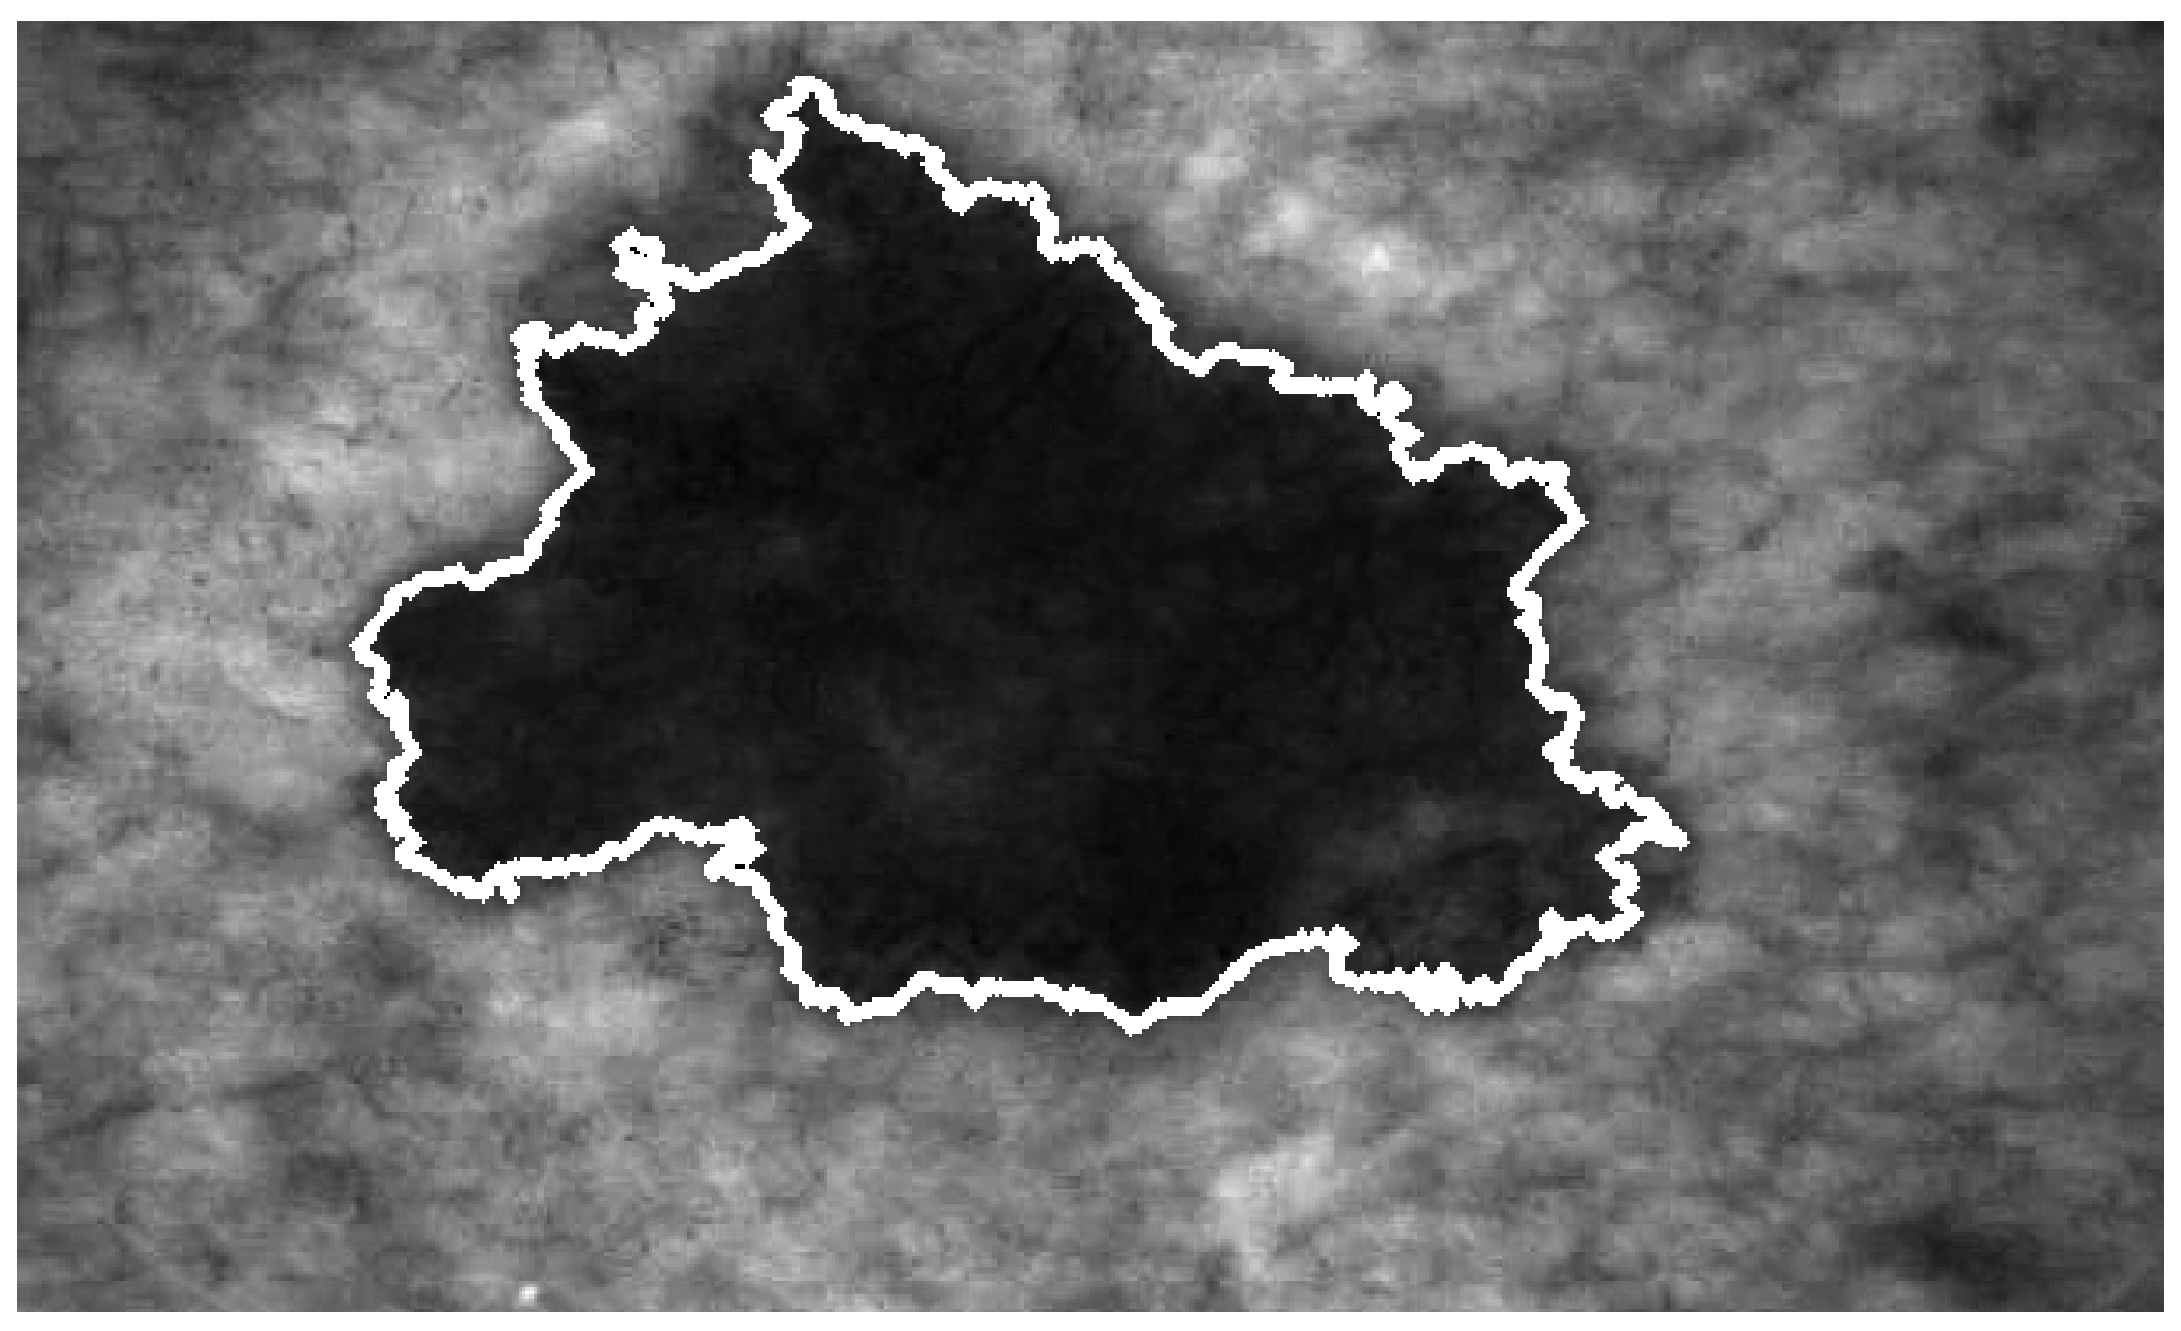
\includegraphics[height = 0.17\textheight, width=0.40\textwidth]{Chapter3/Figures/lesion_border.eps}}
	\hfill
	\subfloat[The \ac{pdf} corresponding to Fig \ref{fig:pdfseg-a}.]{\label{fig:pdfseg-b}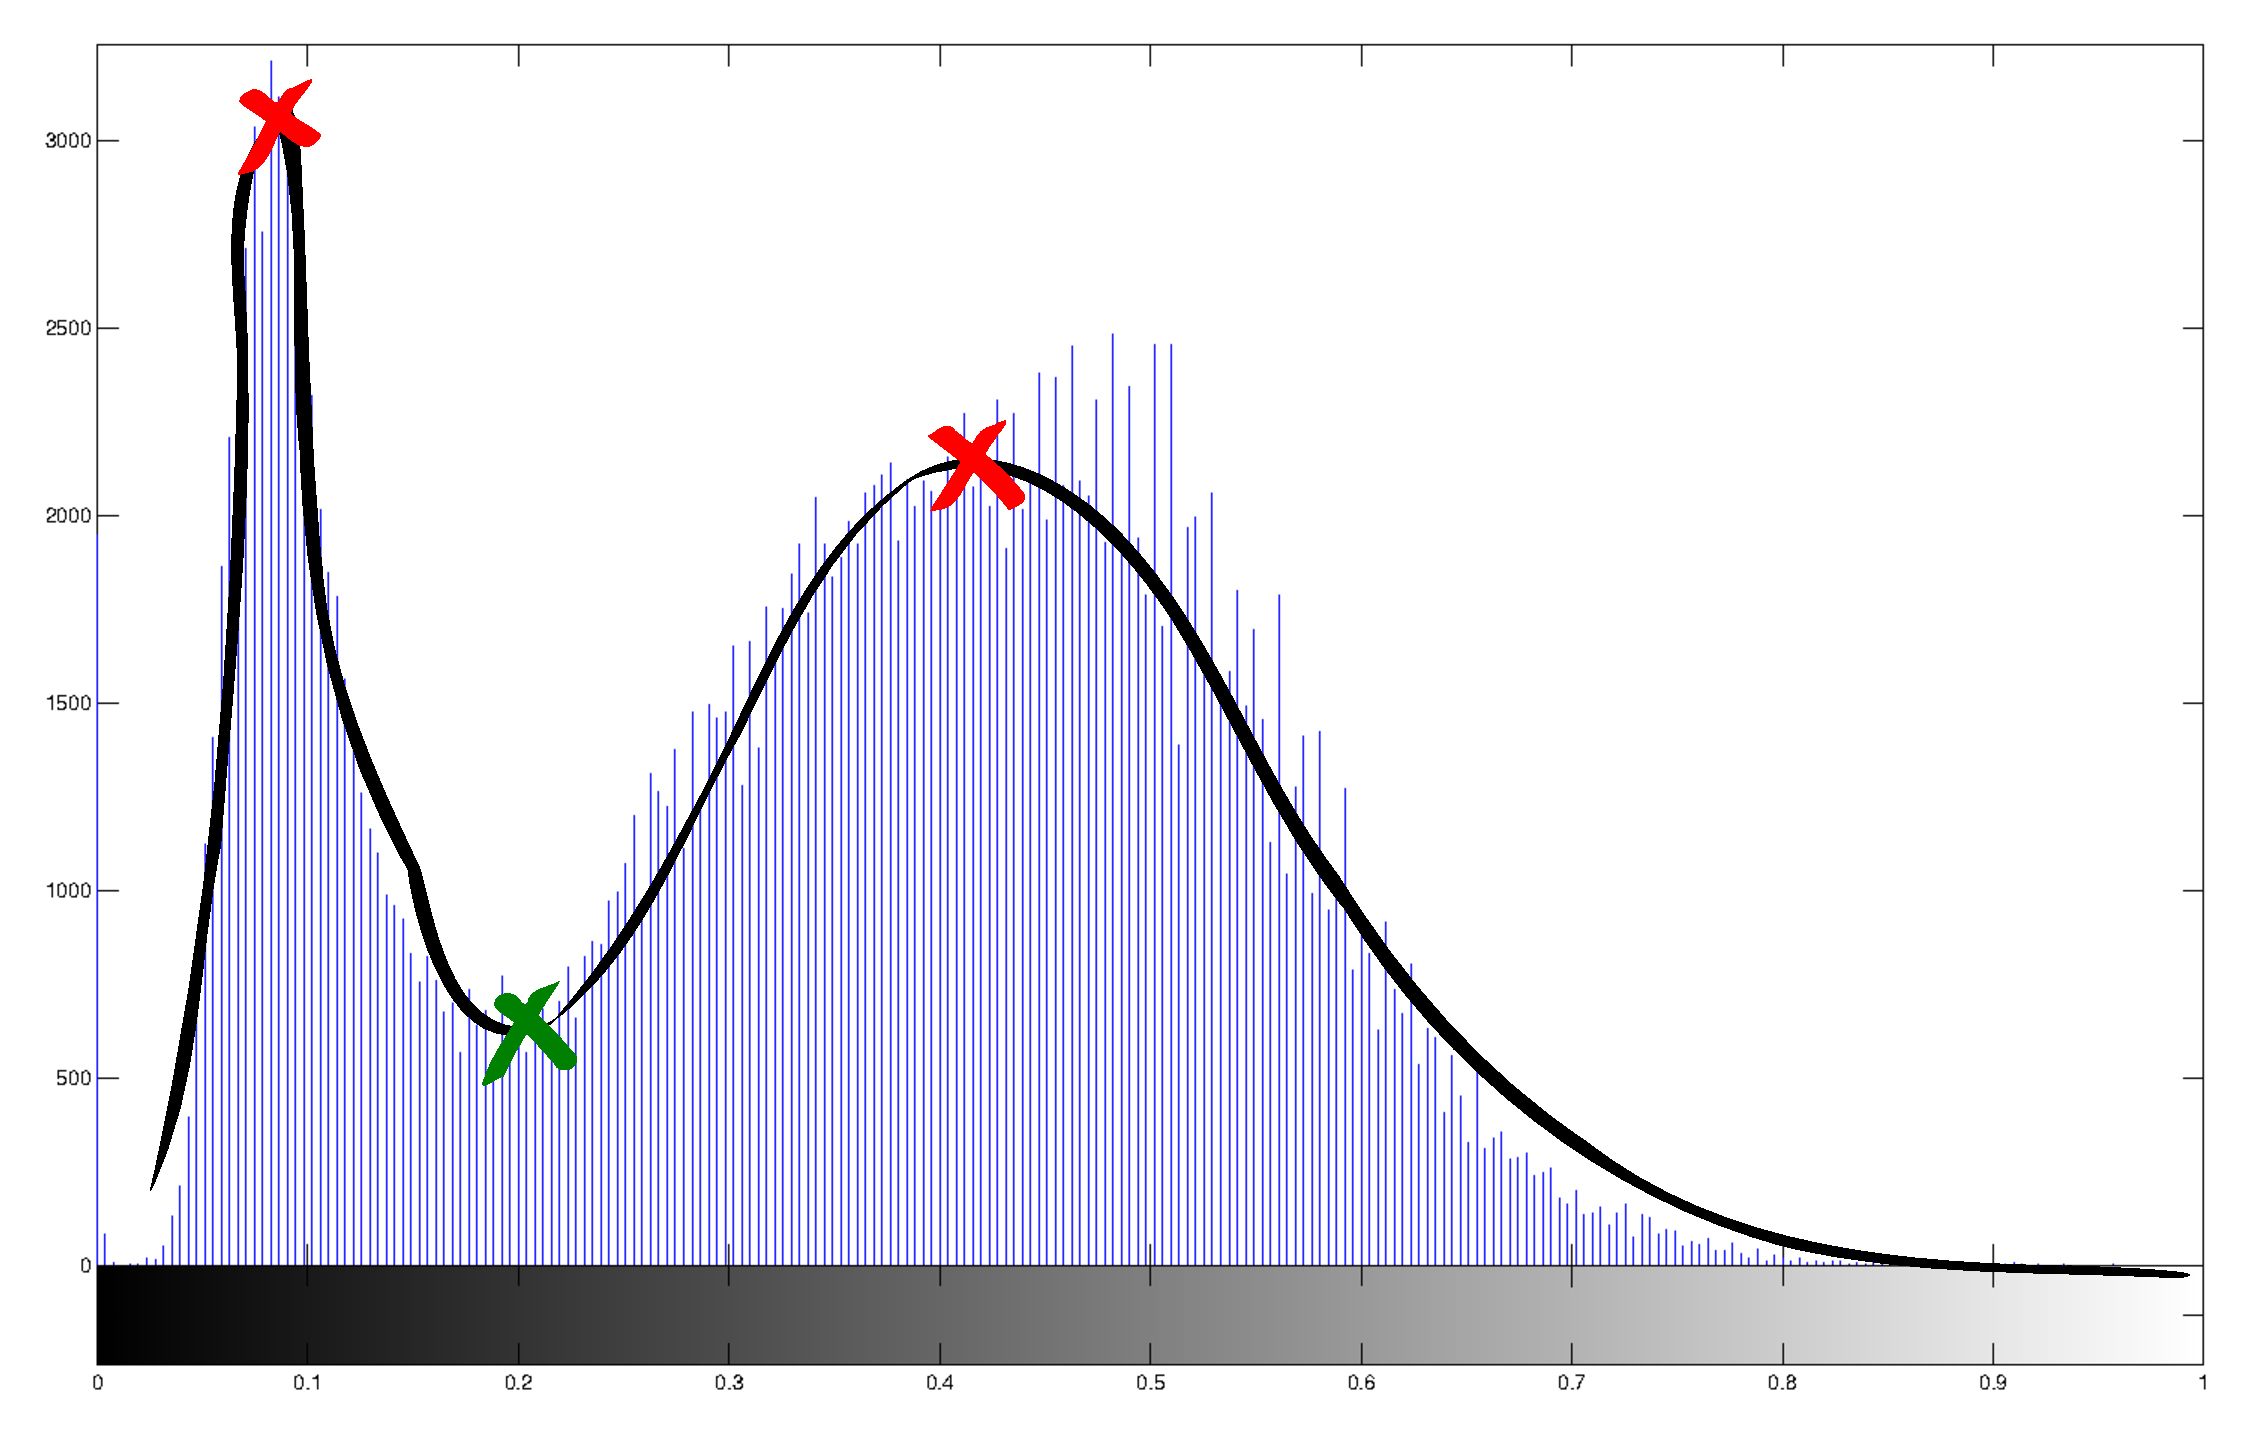
\includegraphics[ height = 0.17\textheight, width=0.40\textwidth]{Chapter3/Figures/ZNomrHist.eps}}
	\hspace*{\fill}
	\caption[\acl{pdf}-based segmentation]{Illustration of the \textit{Z} component (\textit{CIE XYZ} color space) of a dermoscopic image (a) with its corresponding \ac{pdf} (b). The distribution is characterized by a Gaussian mixture with two components. The best threshold is located at the valley between the two Gaussian bells (red cross between the the peaks).
The threshold in this case was found through the peak detetion algorithm and finding the local minium value.}
	\label{fig:pdfseg}
\end{figure}

\noindent Here, the default threshold, considering the utilization of the $Z$-channel, was set to 0.2.
Some results obtained by this algorithm are shown in the second column of Fig.~\ref{fig:plf}.
The lesions in Figs.~\ref{fig:S1a} and~\ref{fig:S1b} are under-segmented, while the lesion in Fig.~\ref{fig:S1d} is over-segmented.
However, the lesions in Figs.~\ref{fig:S1c} and~\ref{fig:S1e} are perfectly delineated.

\item[Level-set methods] are based on the general principle of the active contour, or snakes, approaches~\cite{kass1988snakes}.
These methods looks for a contour of an object by minimizing an energy function, which either uses edge information or region descriptor information.
The level-set method proposed in \cite{li2011level} is region-based because it uses region descriptor as a criterion to guide the motion of the active contour.
If the image domain is illustrated by $\Omega$, the goal of the proposed method is to find a contour $C$, which divides the image into disjoined regions $\{$ $\Omega_{1}, \Omega_{2},..., \Omega_{N}$ $\}$.
The chosen level-set method is suited to our application because it deals with intensity inhomogeneities.
This model defines a local clustering criterion function for the intensities in a circular neighborhood ($\mathcal{O}_{y}$) of each point based on two assumptions: 
(i) the bias image which accounts for intensity inhomogeneities ($b$) is changing slowly and can be approximated by a constant in a neighborhood of each point;
(ii) the pure image without inhomogeneities and noise takes approximately N distinct constant values, $c_{1}, ..., c_{N}$ for N disjoined regions $\Omega_{1}:\Omega_{N}$~\cite{li2011level}.
Based on these assumptions the local clustering criterion function is defined as: 
\begin{equation}
\mathcal{E}_{y} = \sum\limits_{i=1}^{N}\int\limits_{\Omega_{i}} K(y-x)\vert I(x)-b(y)c_{i} \vert^{2} dx~,
\label{eq:ls-lccf}
\end{equation}
\noindent Where $K(y-x)$ is a non-negative window or kernel function equal to 0 for any point outside the neighborhood ($x \notin \mathcal{O}_{y}$).
Considering this function, the optimal partitions ($\Omega_{i}$) of the entire image are defined so that $\mathcal{E}_{y}$ is minimized for all $y$ in the image.
Subsequently, the energy function is taken as the integral of $\mathcal{E}_{y}$ with respect to $y$ in the image domain. 
For the two-phase case (binary) segmentation, the level set energy function is defined as: 
\begin{subequations}
\begin{align}
& \mathcal{E}  = \int \sum\limits_{i=1}^{N}\left( \int K(y-x)\vert I(x) - b(y)c_{i}\vert^{2} dy \right) M_{i}(\phi(x)) dx, \\
& \mathcal{E}(\phi,b,c)  = \int \sum\limits_{i=1}^{N} e_{i}(x) M_{i}(\phi(x)) dx,\\
& e_{i}(x) =  \int K(y-x)\vert I(x) - b(y)c_{i}\vert^{2} dy,\\
& e_{i}(x)  = I^{2}1_{K} - 2c_{i}I(b\ast K)+c_{i}^{2}(b^{2}\ast K).
\label{eq:ls-energy}
\end{align}
\end{subequations}

\noindent The equation above illustrates how to rewrite the energy function in a simplified manner.
The last rows indicate how $e_{i}$ can be computed: $\ast$ is a convolution operation and $1_{K} = \int K(y-x) dy$, which is equal to 1 in the entire image, except near the boundary of the image domain~\cite{li2011level} and $M$ is linked to the Heaviside function.
Using the above energy function, the final level-set formulation is represented as: 
\begin{equation}
\mathcal{F}(\phi,b,c)= \mathcal{E}(\phi,b,c) + \upsilon\mathcal{L}(\phi) + \mu\mathcal{R}(\phi),
\end{equation}
\noindent where $\mathcal{L}(\phi)$ and $\mathcal{R}(\phi)$ are the regularization terms~\cite{li2011level} (see Eq.~\ref{eq:lsLR}).
\begin{subequations}
\begin{align}
\mathcal{L}(\phi) & = \int \vert \nabla H(\phi) \vert dx, \\
\mathcal{R}(\phi) & = \int p(\vert \nabla H(\phi) \vert) dx,\\
p(s) & = (s-1)^{2}/2.
\end{align}
\label{eq:lsLR}
\end{subequations}
\noindent where, $H$ is the unit step (Heaviside) function.

In this research, an initialization region with a bounding box ($200 \times 300$) is considered positioned at center of $Z$-channel.
The $\upsilon$ is set to $0.001 \times 255^{2}$, $\sigma$ is set to 4 and $\mu$ is equal to 1.
These values were set empirically.
The second column of Fig.~\ref{fig:plf} shows some segmentation results achieved by the Level-set method.
As shown, this method segments the lesions perfectly in Fig.~\ref{fig:Oa},~\ref{fig:Ob} and \ref{fig:Od} while it fails to segment the lesions in Fig.~\ref{fig:Oc} and \ref{fig:Oe}.
The difficult and challenging illumination variation and the existing shadows along the left side of the images (Fig.~\ref{fig:Oc} and \ref{fig:Oe}) are the main reasons for the failing in the level-set algorithms.
\begin{figure}
\subfloat[Filter~1]{

\includegraphics[width=0.24\textwidth]{Chapter3/Figures/F1.png}}\hfill
%\subfloat[Filter~2]{
%
\includegraphics[width=0.24\textwidth]{Chapter3/Figures/F2.eps}}\hfill
\subfloat[Filter~2]{

\includegraphics[width=0.24\textwidth]{Chapter3/Figures/F3.png}}\hfill
\subfloat[Filter~3]{

\includegraphics[width=0.24\textwidth]{Chapter3/Figures/F4.png}}
\caption[Fusion filters]{The three main filters for discarding over-segmented and wrongly segmented results prior to fusion.}
\label{fig:segfilters}
\end{figure}

\item[\acl{fcm}] algorithm~\cite{bezdek1984fcm} is a so called soft data clustering approach.
In this technique, contrary to k-\textit{means} algorithms, each data element is described by a set of membership values, which indicate the strength of its association with each cluster.
This membership value is referred to as an association probability between data elements and clusters.
Fuzzy clustering uses these memberships to assign the elements to their closest cluster.
Considering a set of data elements, $X=\{x_{1},...,x_{n}\}$, and a list of clusters, $C= \{c_{1}, ...,c_{K}\}$, a partition matrix $W_{n\times k}= \{w_{ij} \in [0,1]\}$ is defined so that each of its elements $w_{ij}$ show the degree to which an element $x_{i}$ belongs to cluster $c_{j}$.
Thus, the \ac{fcm} intends to minimize the following cost:
\begin{subequations}
\begin{align}
& \min\limits_{c} \sum\limits_{i=1}^{n}\sum\limits_{j=1}^{K} w_{ij}^{m}\Vert x_{i}-c_{j} \Vert^{2}~,\\
& w_{ij}^{m} = \frac{1}{\sum\limits_{k=1}^{K} \left(\frac{\Vert x_{i} -c_{j} \Vert}{\Vert x_{i} -c_{k} \Vert}\right)^{2/m-1}}~,
\end{align}
\end{subequations}
\noindent The $m$ is called the fuzzifier ($m\geq 1$).
Larger values of $m$ lead to a smaller membership and thus a fuzzier clustering~\cite{bezdek1984fcm}.

In this study, we performed \ac{fcm} clustering with $K=2$, and $m = 2.0$ on the $Z$-channel of each image. 
The third column of Fig.~\ref{fig:plf} shows the segmentation results obtained with the \ac{fcm} algorithm.
This algorithm segments the lesions perfectly in Fig.~\ref{fig:Oa},~\ref{fig:Ob},~\ref{fig:Oc}, and~\ref{fig:Od}.
However, it fails to segment the last lesion in Fig.~\ref{fig:Oe}.

\item[Segmentation fusion] is considered as combining the segmented results from the three algorithms into one final result.
As shown in Fig.\,\ref{fig:plf}, each algorithm often under-segments (Fig.\,\ref{fig:S1b}), over-segments (Fig.\,\ref{fig:S1d},\,\ref{fig:S3e}) or wrongly identifies some lesions (Fig.\,\ref{fig:S2c}).

Although under-segmentation is not a problem and can be corrected by fusion methods, it is preferable to avoid over-segmented or wrongly-segmented results.
Also, the initial experiments with the Vienna dataset indicated that often only one algorithm performs correctly while the other two fail.
Thus, the majority voting or any other fusion method, such as \acs{staple}, will not perform efficiently without some preliminary filtering steps.


In this regard, some basic filtering steps are proposed to identify the wrong and over segmented results.
Three main filters are used, shown in Fig.~\ref{fig:segfilters}.
Prior to applying the filters, the images are first divided into two groups: the first group, the majority group, contains images which the lesions do not touch the borders of the images.
The second group, the minority group, contains images of larger lesions.
These lesions usually cover the entire image and are connected to the border.
Through primary observation it was concluded that the level-set algorithm segments these lesions perfectly.
Subsequently, for this group, only this algorithm is used.

While for the former group, the segmented result is multiplied to each of the filters and the number of common pixels between them are measured.
This measurement defines a connectivity index ($CI$) between each filter and a segmented result.
Thus, if the segmented results have a high $CI$ with respect to filter~1 and 2 (higher than 60\%), the result is discarded as over-segmented and if it only has a high $CI$ with respect to filter~3 (over 40\%), it is considered as a wrong segmentation.
After discarding the undesired segmentations for each image, the remaining segmentations are added together.
If one or none of the segmentation results are discarded, the final result is based on majority voting of two among all three and if two of them are discarded, the final result is equal to the remaining segmentation.

%Obviously, based on the proposed fusion algorithm, the segmentation of larger lesions which cover the entire image, will be discarded in the filtering step.
%Through the primary experiments it was observed that larger lesions were best segmented with level-set algorithm.
%Thus we considered dividing the images into two categories, the smaller lesions which belong to a larger portion of the dataset were segmented through the fusion algorithm.
%However the larger lesions segmented with level-set.
%First we divide the images into two categories, the first one contains the images of large lesions which almost cover the entire image, and the second group contains the rest of the images.
%During the experiments, it was observed that level-set performs the best for the first group, while pdf-based fails to find the best threshold.  
\end{description}



\begin{figure}
\begin{center}
\subfloat[]{\label{fig:Oa}
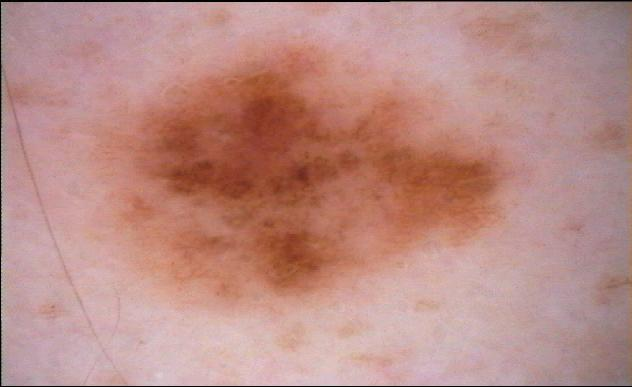
\includegraphics[scale=0.15]{Chapter3/Figures/D605.jpg}}\
\subfloat[]{\label{fig:S1a}
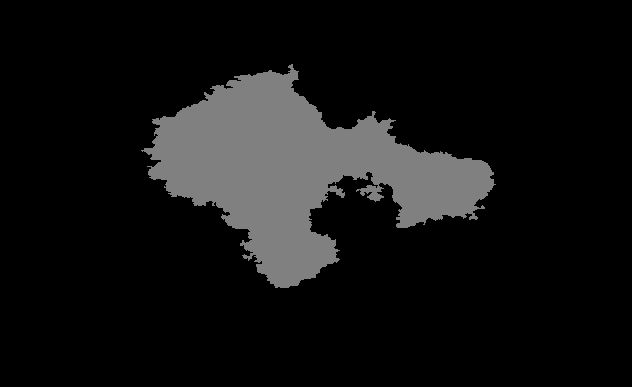
\includegraphics[scale=0.15]{Chapter3/Figures/D605-mask_pdf.png}}\
\subfloat[]{\label{fig:S2a}
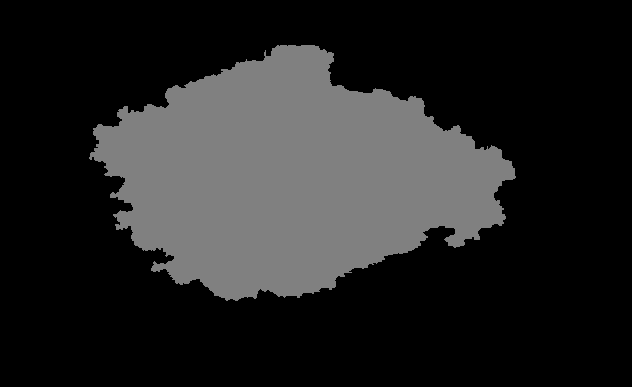
\includegraphics[scale=0.15]{Chapter3/Figures/D605-mask_LS.png}}\
\subfloat[]{\label{fig:S3a}
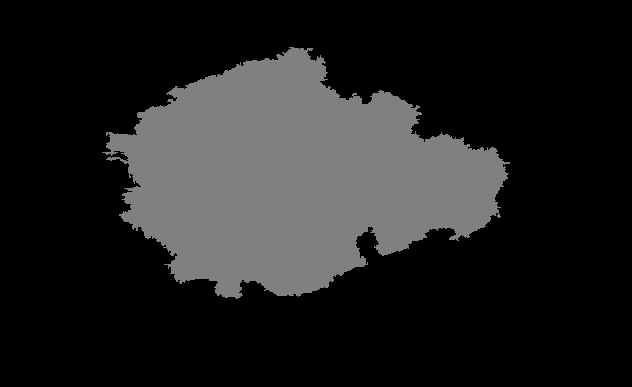
\includegraphics[scale=0.15]{Chapter3/Figures/D605-mask_FC.png}}\\
\subfloat[]{\label{fig:Ob}
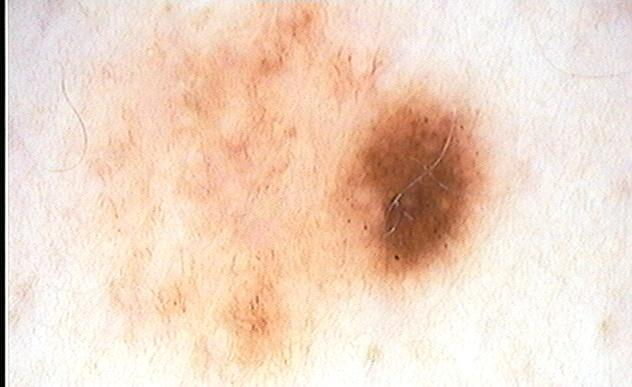
\includegraphics[scale=0.15]{Chapter3/Figures/D26.jpg}}\
\subfloat[]{\label{fig:S1b}
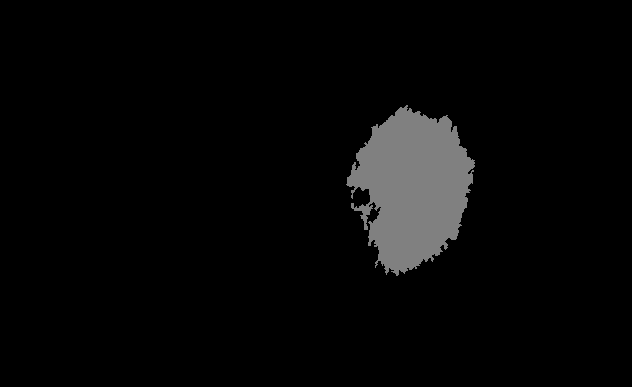
\includegraphics[scale=0.15]{Chapter3/Figures/D26-mask_pdf.png}}\
\subfloat[]{\label{fig:S2b}
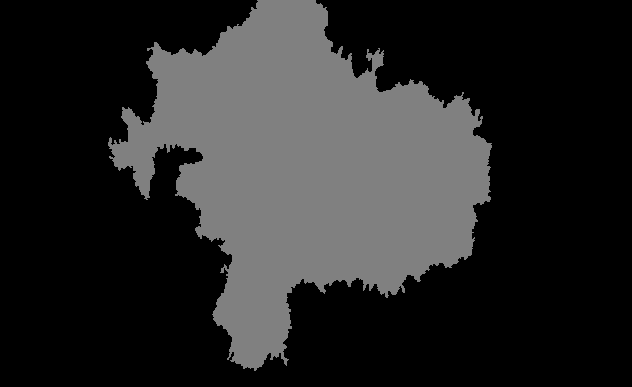
\includegraphics[scale=0.15]{Chapter3/Figures/D26-mask_LS.png}}\
\subfloat[]{\label{fig:S3b}
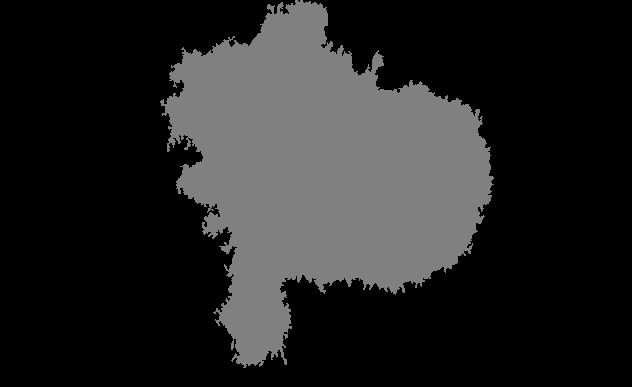
\includegraphics[scale=0.15]{Chapter3/Figures/D26-mask_FC.png}}\\
\subfloat[]{\label{fig:Oc}
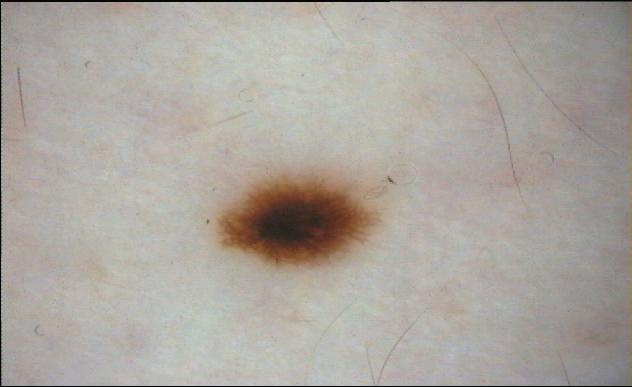
\includegraphics[scale=0.15]{Chapter3/Figures/D117.jpg}}\
\subfloat[]{\label{fig:S1c}
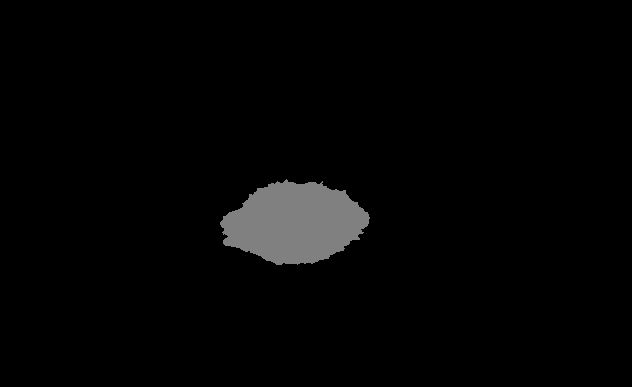
\includegraphics[scale=0.15]{Chapter3/Figures/D117-mask_pdf.png}}\
\subfloat[]{\label{fig:S2c}
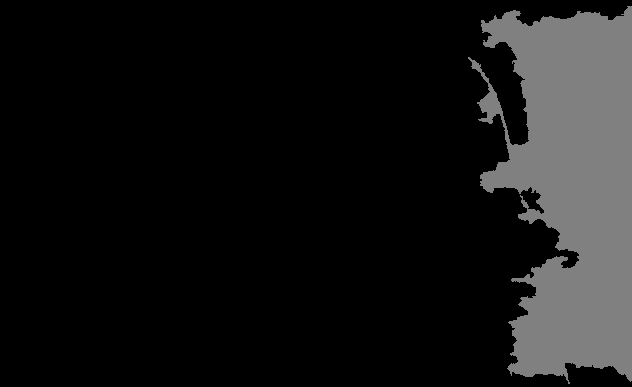
\includegraphics[scale=0.15]{Chapter3/Figures/D117-mask_LS.png}}\
\subfloat[]{\label{fig:S3c}
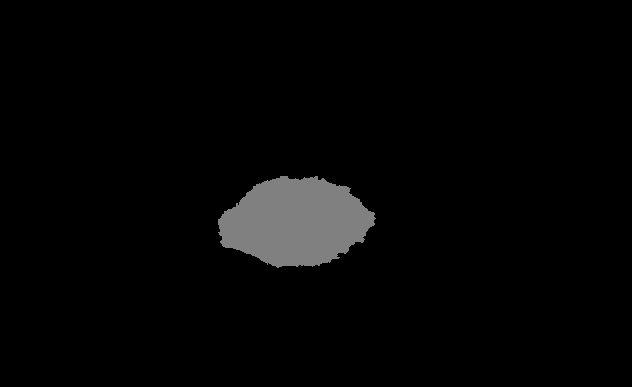
\includegraphics[scale=0.15]{Chapter3/Figures/D117-mask_FC.png}}\\
\subfloat[]{\label{fig:Od}
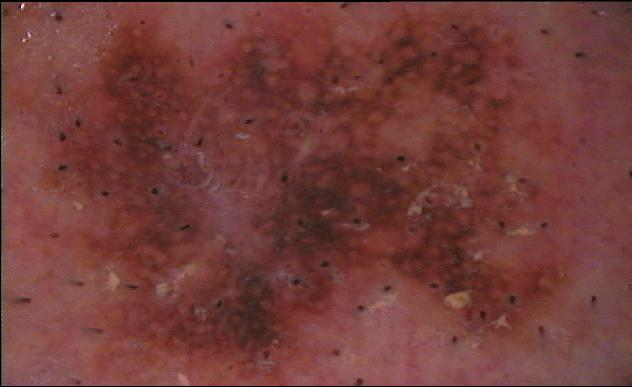
\includegraphics[scale=0.15]{Chapter3/Figures/G781.jpg}}\
\subfloat[]{\label{fig:S1d}

\includegraphics[scale=0.15]{Chapter3/Figures/G781-mask_pdf.png}}\
\subfloat[]{\label{fig:S2d}
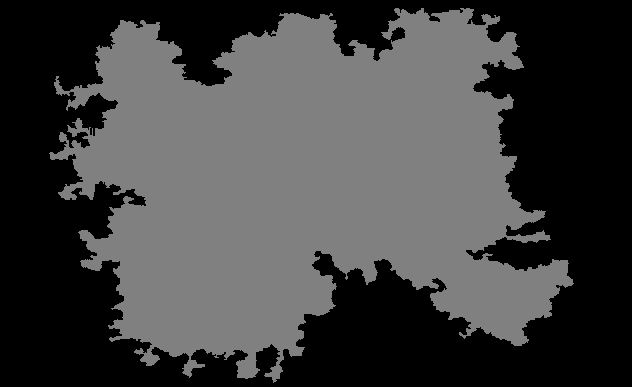
\includegraphics[scale=0.15]{Chapter3/Figures/G781-mask_LS.png}}\
\subfloat[]{\label{fig:S3d}
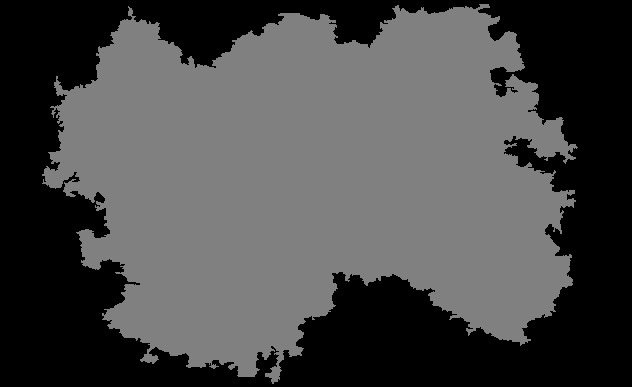
\includegraphics[scale=0.15]{Chapter3/Figures/G781-mask_FC.png}}\\
\subfloat[]{\label{fig:Oe}
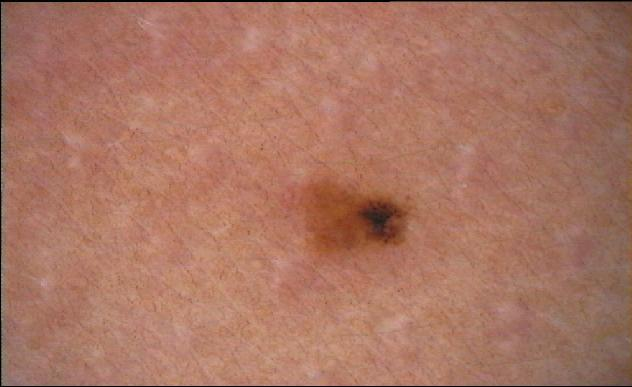
\includegraphics[scale=0.15]{Chapter3/Figures/D538.jpg}}\
\subfloat[]{\label{fig:S1e}
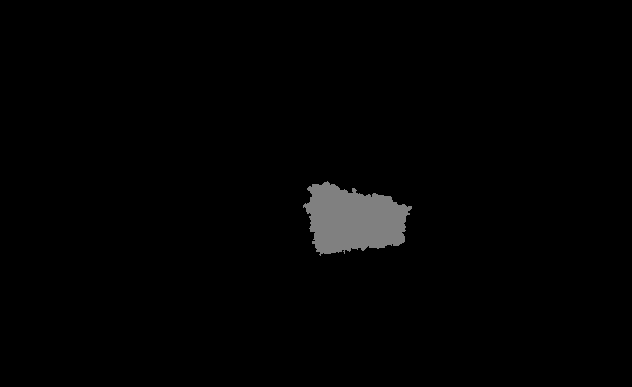
\includegraphics[scale=0.15]{Chapter3/Figures/D538-mask_pdf.png}}\
\subfloat[]{\label{fig:S2e}
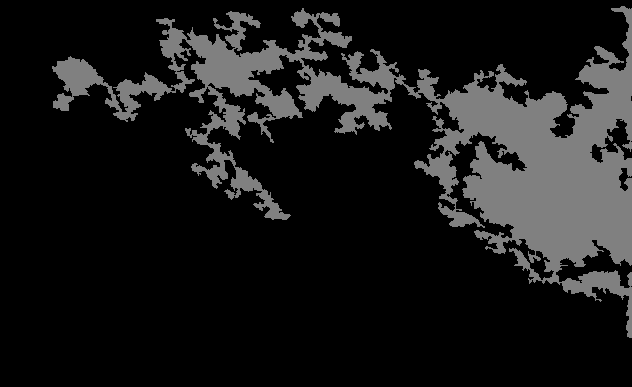
\includegraphics[scale=0.15]{Chapter3/Figures/D538-mask_LS.png}}\
\subfloat[]{\label{fig:S3e}

\includegraphics[scale=0.15]{Chapter3/Figures/D538-mask_FC.png}}\
\end{center}
\caption[Segmentation results obtained by the \ac{pdf}-based, level-set and \ac{fcm} algorithms]{Segmentation results obtained by the \ac{pdf}-based, level-set and \ac{fcm} algorithms (second, third and forth columns from the left, respectively). The original images are shown in the leftmost column.
In order to avoid the influence of the black border in the original images, the segmentation methods ignore 15 pixels along the borders of each image.
The results in rows 3--5 demonstrate the methods' failures.}
\label{fig:plf}
\end{figure} 


